\begin{hcarentry}[updated]{GenI}
\label{geni}
\report{Eric Kow}%05/09
\makeheader

GenI is a surface realizer for Tree Adjoining Grammars.  Surface
realization can be seen a subtask of natural language generation
(producing natural language utterances, eg. English texts, out of
abstract inputs).  GenI in particular takes an FB-LTAG grammar and an
input semantics (a conjunction of first order terms), and produces the
set of sentences associated to the input semantics by the grammar.  It
features a surface realization library, several optimizations, batch
generation mode, and a graphical debugger written in wxHaskell.  It was
developed within the TALARIS project and is free software licensed under
the GNU GPL.

%**<img src="./GenI-main-screenshot.jpg">
%*ignore
\begin{center}
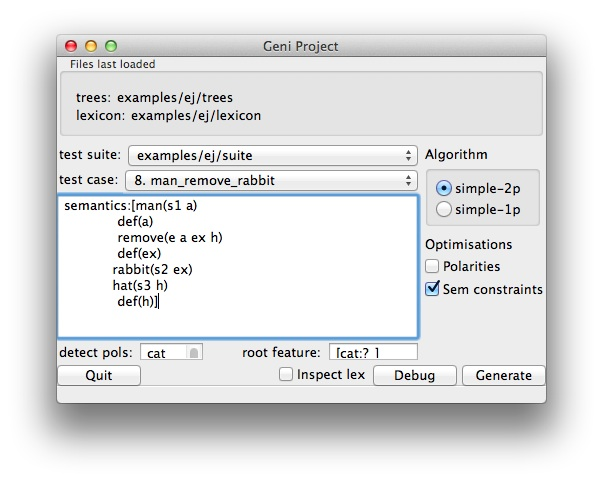
\includegraphics[width=0.47\textwidth]{html/GenI-main-screenshot.jpg}
\end{center}
%*endignore

%**<img src="./GenI-debugger-screenshot.jpg">
%*ignore
\begin{center}
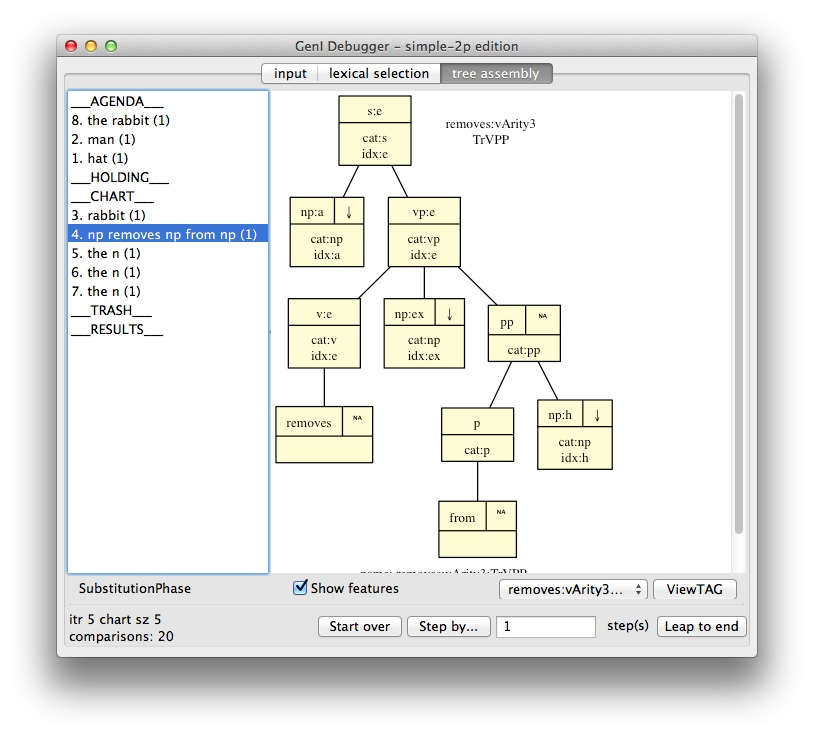
\includegraphics[width=0.47\textwidth]{html/GenI-debugger-screenshot.jpg}
\end{center}
%*endignore

GenI is available on Hackage, and can be installed via cabal-install.
Our most recent release of GenI was version 0.20.1 (2009-10-01), which
offers cleaner interactions with the third-party tools (using JSON),
simpler installation on MacOS X and a user manual.  For more
information, please contact us on the geni-users mailing list.

\FurtherReading
\begin{compactitem}
\item \url{http://projects.haskell.org/GenI}
\item Paper from Haskell Workshop 2006:

\url{http://hal.inria.fr/inria-00088787/en}
\item \url{http://websympa.loria.fr/wwsympa/info/geni-users}
\end{compactitem}
\end{hcarentry}
